\documentclass{if-beamer}

% --------------------------------------------------- %
%                  Presentation info	              %
% --------------------------------------------------- %
\title[Lecture 14]{Lecture 14}
\subtitle{Optimization}
\author{Ashley Gannon}
\date{ISC3313 Fall 2021}
\logo{

\includegraphics[scale=0.08]{figures/FSULogo.png}
}
\subject{Presentation subject}

% --------------------------------------------------- %
%                    Title + Schedule                 %
% --------------------------------------------------- %
\begin{document}

\begin{frame}
  \titlepage
\end{frame}
% --------------------------------------------------- %
%                      Presentation                   %
% --------------------------------------------------- %
\section{What is optimization?}

\begin{frame}[t]
	\frametitle{What is optimization?}
	\begin{itemize}
		\item The determination of a function's maximum or minimum (or optimal) value is referred to as \textit{optimization}.
	\end{itemize}
\end{frame}

\begin{frame}[t]
	\frametitle{What is optimization?}
	\begin{itemize}
		\item The determination of a function's maximum or minimum (or optimal) values is referred to as \textit{optimization}.
		\item  As you learned in calculus, such solutions can be obtained analytically by determining the value at which the function is flat; $f'(x) = 0$.
	\end{itemize}
\end{frame}

\begin{frame}[t]
	\frametitle{What is optimization?}
	\begin{itemize}
		\item The determination of a function's maximum or minimum (or optimal) value is referred to as \textit{optimization}.
		\item  As you learned in calculus, such solutions can be obtained analytically by determining the value at which the function is flat; $f'(x) = 0$.
		\item The fundemental difference is that finding the location of a root  involves searching for $x$ where the $f(x) = 0$ while optimization involves searching for $x$ where $f'(x) = 0$.
		\begin{figure}
			\centering
			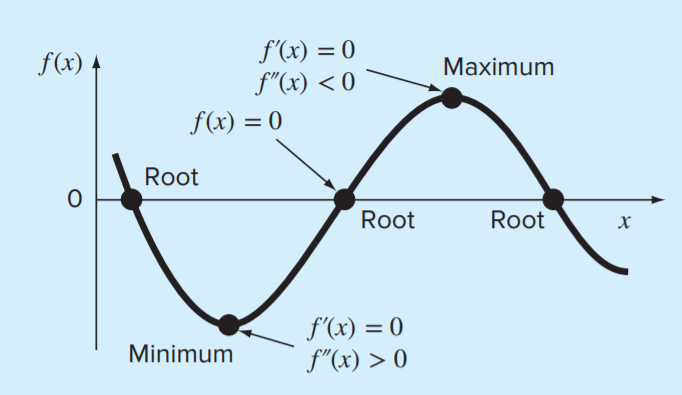
\includegraphics[width=.4\textwidth]{figures/optimavsroot}
		\end{figure}
	\end{itemize}
\end{frame}

\begin{frame}
		\frametitle{Optimization Example}
Let's consider the following problem: \\\vspace{8pt}
An object like a bungee jumper can be projected upward at a specified velocity. If it is subject to linear drag, its altitude as a function of time can be computed as
$$ z = z_0 +\frac{m}{c_d}\left(v_0+\frac{mg}{c_d}\right)\left(1-e^{\frac{-c_dt}{m}}\right) -\frac{mg}{c_d}t $$
Where $z$ is the distance from the Earth's surface, $z_0$ is the initial distance from the earths surface, $v_0$ is the initial velocity, $m$ is the mass of the jumper, $c_d$ is the drag coefficient, and $t$ is time. 
\end{frame}

\begin{frame}
	\frametitle{Optimization Example}
	Let's consider the following problem: \\\vspace{8pt}
	An object like a bungee jumper can be projected upward at a specified velocity. If it is subject to linear drag, its altitude as a function of time can be computed as
	$$ z = z_0 +\frac{m}{c_d}\left(v_0+\frac{mg}{c_d}\right)\left(1-e^{\frac{-c_dt}{m}}\right) -\frac{mg}{c_d}t $$
	If we let $z_0 = 100$m, $m = 80$kg, $c_d = 15$kg/s, $v_0 = 55$m/s, and $g = 9.81$m/$\textrm{s}^2$, and plot $z$ for $t = 0...12$
	\begin{figure}
		\centering
		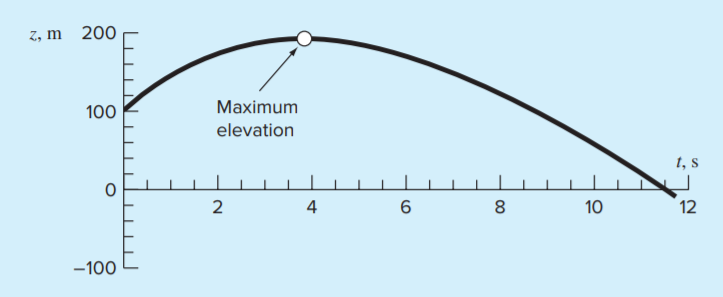
\includegraphics[width=.8\textwidth]{figures/graphex}
	\end{figure}
\end{frame}

\begin{frame}
	\frametitle{Optimization Example}
	Let's consider the following problem: \\\vspace{8pt}
	An object like a bungee jumper can be projected upward at a specified velocity. If it is subject to linear drag, its altitude as a function of time can be computed as
	$$ z = z_0 +\frac{m}{c_d}\left(v_0+\frac{mg}{c_d}\right)\left(1-e^{\frac{-c_dt}{m}}\right) -\frac{mg}{c_d}t $$
	To find the maximum altitude analytically, we have to find the time where $z'(t) = 0$.
	$$\frac{dz}{dt} = v_0e^{\frac{-c_dt}{m}} - \frac{mg}{c_d}\left( 1-e^{\frac{-c_dt}{m}} \right)=0$$
\end{frame}

\begin{frame}
	\frametitle{Optimization Example}
	Let's consider the following problem: \\\vspace{8pt}
	An object like a bungee jumper can be projected upward at a specified velocity. If it is subject to linear drag, its altitude as a function of time can be computed as
	$$ z = z_0 +\frac{m}{c_d}\left(v_0+\frac{mg}{c_d}\right)\left(1-e^{\frac{-c_dt}{m}}\right) -\frac{mg}{c_d}t $$
	To find the maximum altitude analytically, we have to find the time where $z'(t) = 0$.
	$$\frac{dz}{dt} = v_0e^{\frac{-c_dt}{m}} - \frac{mg}{c_d}\left(1-e^{\frac{-c_dt}{m}}\right)=0$$
	Solving analytically for $t$ we get
	$$ t = \frac{m}{c_d}\ln\left(1+\frac{c_dv_0}{mg} \right) $$
\end{frame}

\begin{frame}
	\frametitle{Optimization Example}
	Let's consider the following problem: \\\vspace{8pt}
	An object like a bungee jumper can be projected upward at a specified velocity. If it is subject to linear drag, its altitude as a function of time can be computed as
	$$ z = z_0 +\frac{m}{c_d}\left(v_0+\frac{mg}{c_d}\right)\left(1-e^{\frac{-c_dt}{m}}\right) -\frac{mg}{c_d}t $$
	To find the maximum altitude analytically, we have to find the time where $z'(t) = 0$.
	$$\frac{dz}{dt} = v_0e^{\frac{-c_dt}{m}} - \frac{mg}{c_d}\left(1-e^{\frac{-c_dt}{m}}\right)=0$$
	Solving analytically for $t$ we get
	$$ t = \frac{m}{c_d}\ln\left(1+\frac{c_dv_0}{mg} \right) $$
	Again, letting $z_0 = 100$m, $m = 80$kg, $c_d = 15$kg/s, $v_0 = 55$m/s, and $g = 9.81$m/$\textrm{s}^2$
	$$ t \approx 3.83166\textrm{s}$$
\end{frame}

\begin{frame}
	\frametitle{Optimization Example}
	Now to find the maximum position, we plug this value for $t$ and our other parameters back into 
		$$ z = z_0 +\frac{m}{c_d}\left(v_0+\frac{mg}{c_d}\right)\left(1-e^{\frac{-c_dt}{m}}\right) -\frac{mg}{c_d}t $$
	to find that 
	$$ z \approx 192.8609 \textrm{m}$$
\end{frame}

\begin{frame}
	\frametitle{Optimization Example}
	Now to find the maximum position, we plug this value for $t$ and our other parameters back into 
	$$ z = z_0 +\frac{m}{c_d}\left(v_0+\frac{mg}{c_d}\right)\left(1-e^{\frac{-c_dt}{m}}\right) -\frac{mg}{c_d}t $$
	to find that 
	$$ z \approx 192.8609 \textrm{m}$$
	Now if we want to verify that this is a maximum value, we need to evaluate $z''(x)$
	$$\frac{dz^2}{d^2z} = -\frac{c_dv_0}{m}e^{\frac{-c_dt}{m}} -ge^{\frac{-c_dt}{m}}$$
\end{frame}

\begin{frame}
	\frametitle{Optimization Example}
	Now to find the maximum position, we plug this value for $t$ and our other parameters back into 
	$$ z = z_0 +\frac{m}{c_d}\left(v_0+\frac{mg}{c_d}\right)\left(1-e^{\frac{-c_dt}{m}}\right) -\frac{mg}{c_d}t $$
	to find that 
	$$ z \approx 192.8609 \textrm{m}$$
	Now if we want to verify that this is a maximum value, we need to evaluate $z''(x)$
	$$\frac{dz^2}{d^2z} = -\frac{c_dv_0}{m}e^{\frac{-c_dt}{m}} -ge^{\frac{-c_dt}{m}}$$
	plugging in our variable values, 
	$$\frac{dz^2}{d^2z} \approx -9.81 \textrm{m/s}$$
	The fact that the second derivative is negative tells us that we have a maximum. 
\end{frame}

\begin{frame}[t]
	\frametitle{What is optimization?}
	\begin{itemize}
		\item The determination of a function's maximum or minimum (or optimal) value is referred to as \textit{optimization}.
		\item  As you learned in calculus, such solutions can be obtained analytically by determining the value at which the function is flat; $f'(x) = 0$.
		\item The fundemental difference is that finding the location of a root  involves searching for $x$ where the $f(x) = 0$ while optimization involves searching for $x$ where $f'(x) = 0$.
		\begin{figure}
			\centering
			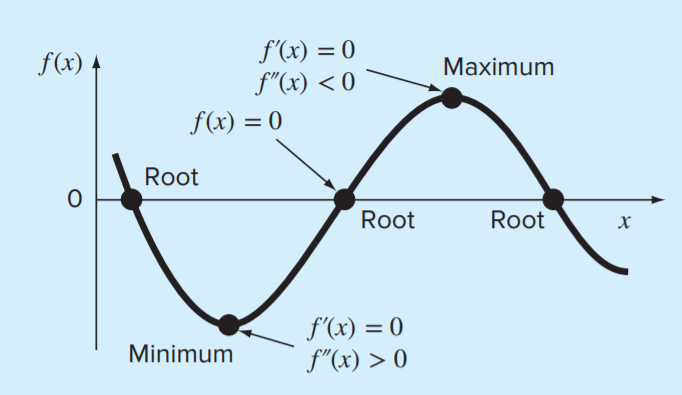
\includegraphics[width=.4\textwidth]{figures/optimavsroot}
		\end{figure}
		\item Although such analytical solutions are sometimes feasible, most practical optimization problems require numerical, computer solutions.
	\end{itemize}
\end{frame}

\begin{frame}[t]
\frametitle{What is optimization?}
\begin{itemize}
	\item The determination of a function's maximum or minimum (or optimal) value is referred to as \textit{optimization}.
	\item  As you learned in calculus, such solutions can be obtained analytically by determining the value at which the tangent of the function is flat; $f'(x) = 0$.
	\item The fundemental difference is that finding the location of a root  involves searching for $x$ where the $f(x) = 0$ while optimization involves searching for $x$ where $f'(x) = 0$.
	\begin{figure}
		\centering
		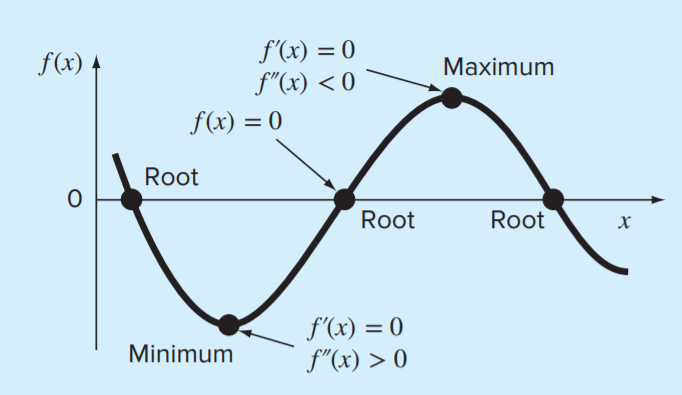
\includegraphics[width=.4\textwidth]{figures/optimavsroot}
	\end{figure}
	\item Although such analytical solutions are sometimes feasible, most practical optimization problems require numerical, computer solutions.
	\item From a numerical standpoint, such optimization methods are similar in spirit to the root-location methods we discussed in the last section.
	\begin{itemize}
		\item both involve guessing and searching for a location on a continuous function.
	\end{itemize}

\end{itemize}
\end{frame}

\section{One Dimensional Optimization}
\begin{frame}[t]
	\frametitle{1D Optimization}
	\begin{itemize}
		\item In this unit we will cover techniques that find the minimum or maximum of a function of a single variable, i.e. $f(x)$.
	\end{itemize}
\end{frame}

\begin{frame}[t]
	\frametitle{1D Optimization}
	\begin{itemize}
		\item In this unit we will cover techniques that find the minimum or maximum of a function of a single variable, i.e. $f(x)$.
		\item Just as finding the root location was complicated by the fact that several roots can occur for a single function, both local
		and global optima can occur in optimization.
		\begin{figure}
			\centering
			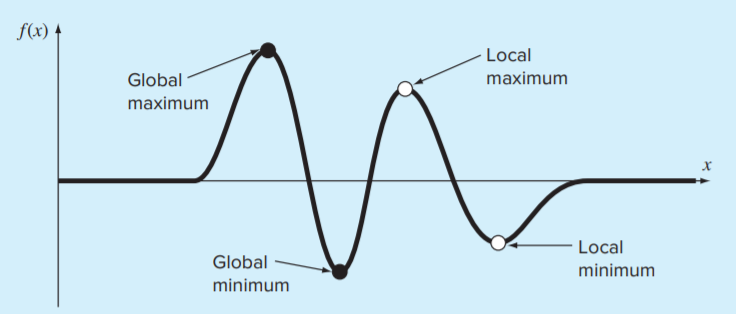
\includegraphics[width = 0.65\textwidth]{figures/localglobal}
		\end{figure}
	\end{itemize}
\end{frame}

\begin{frame}[t]
	\frametitle{1D Optimization}
	\begin{itemize}
		\item In this unit we will cover techniques that find the minimum or maximum of a function of a single variable, i.e. $f(x)$.
		\item Just as finding the root location was complicated by the fact that several roots can occur for a single function, both local
		and global optima can occur in optimization.
		\begin{figure}
			\centering
			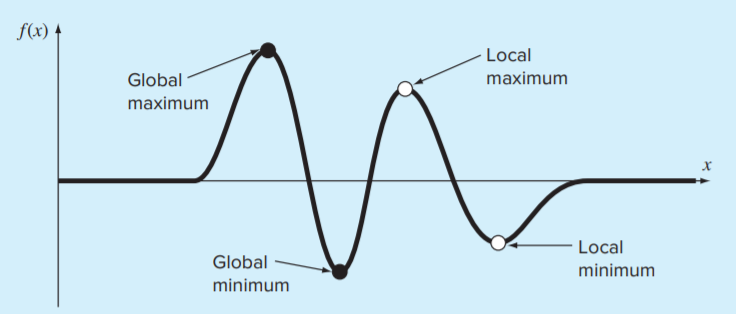
\includegraphics[width = 0.65\textwidth]{figures/localglobal}
		\end{figure}
		\begin{itemize}
			\item A \textit{global} optimum represents the very best solution. 
		\end{itemize}
	\end{itemize}
\end{frame}

\begin{frame}[t]
	\frametitle{1D Optimization}
	\begin{itemize}
		\item In this unit we will cover techniques that find the minimum or maximum of a function of a single variable, i.e. $f(x)$.
		\item Just as finding the root location was complicated by the fact that several roots can occur for a single function, both local
		and global optima can occur in optimization.
		\begin{figure}
			\centering
			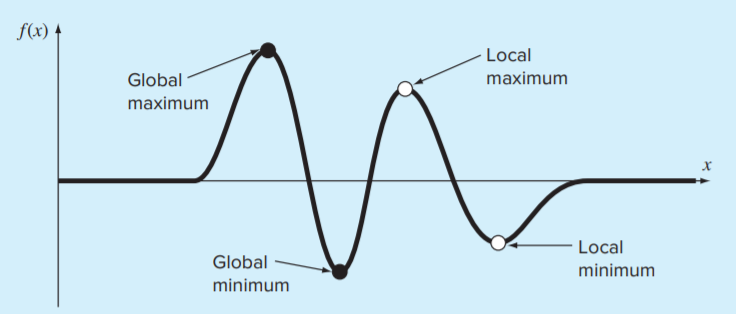
\includegraphics[width = 0.65\textwidth]{figures/localglobal}
		\end{figure}
		\begin{itemize}
			\item A \textit{global} optimum represents the very best solution. 
			\item A \textit{local} optimum, though not the very best, is better than its immediate neighbors. 
		\end{itemize}
	\end{itemize}
\end{frame}

\begin{frame}[t]
	\frametitle{1D Optimization}
	\begin{itemize}
		\item In this unit we will cover techniques that find the minimum or maximum of a function of a single variable, i.e. $f(x)$.
		\item Just as finding the root location was complicated by the fact that several roots can occur for a single function, both local
		and global optima can occur in optimization.
		\begin{figure}
			\centering
			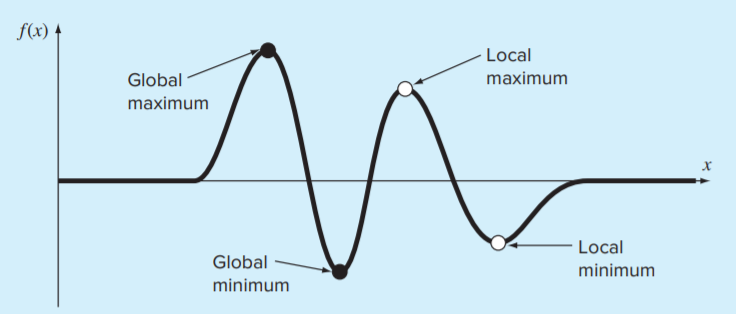
\includegraphics[width = 0.65\textwidth]{figures/localglobal}
		\end{figure}
		\begin{itemize}
			\item A \textit{global} optimum represents the very best solution. 
			\item A \textit{local} optimum, though not the very best, is better than its immediate neighbors. 
			\item Cases that include local optima are called \textit{multimodal}. 
		\end{itemize}
	\end{itemize}
\end{frame}

\begin{frame}[t]
	\frametitle{1D Optimization}
	\begin{itemize}
		\item In this unit we will cover techniques that find the minimum or maximum of a function of a single variable, i.e. $f(x)$.
		\item Just as finding the root location was complicated by the fact that several roots can occur for a single function, both local
		and global optima can occur in optimization.
		\begin{figure}
			\centering
			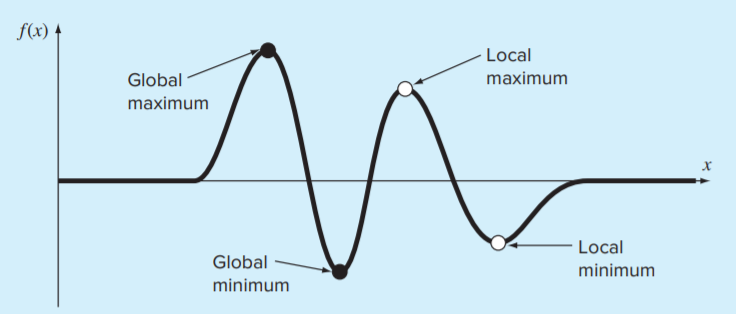
\includegraphics[width = 0.65\textwidth]{figures/localglobal}
		\end{figure}
		\begin{itemize}
			\item A \textit{global} optimum represents the very best solution. 
			\item A \textit{local} optimum, though not the very best, is better than its immediate neighbors. 
			\item Cases that include local optima are called \textit{multimodal}. 
			\item In such cases, we will almost always be interested in finding the global optimum. 
		\end{itemize}
	\end{itemize}
\end{frame}

\begin{frame}[t]
	\frametitle{1D Optimization}
	\begin{itemize}
		\item In this unit we will cover techniques that find the minimum or maximum of a function of a single variable, i.e. $f(x)$.
		\item Just as finding the root location was complicated by the fact that several roots can occur for a single function, both local
		and global optima can occur in optimization.
		\begin{figure}
			\centering
			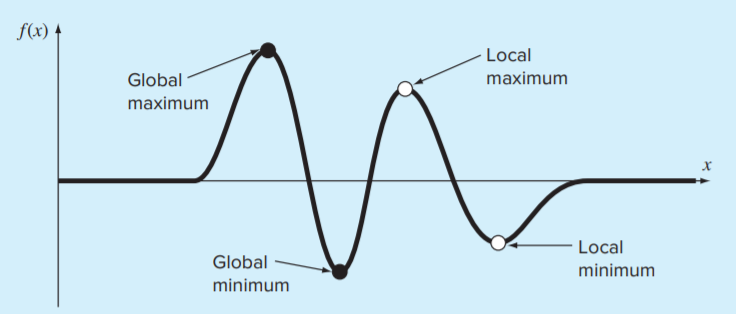
\includegraphics[width = 0.65\textwidth]{figures/localglobal}
		\end{figure}
		\begin{itemize}
			\item A \textit{global} optimum represents the very best solution. 
			\item A \textit{local} optimum, though not the very best, is better than its immediate neighbors. 
			\item Cases that include local optima are called \textit{multimodal}. 
			\item In such cases, we will almost always be interested in finding the global optimum.
			\item Therfore, we must be concerned about mistaking a local result for the global optimum. 
		\end{itemize}
	\end{itemize}
\end{frame}

\begin{frame}[t]
	\frametitle{1D Optimization}
	\begin{itemize}
		\item In this unit we will cover techniques that find the minimum or maximum of a function of a single variable, i.e. $f(x)$.
		\item Just as finding the root location was complicated by the fact that several roots can occur for a single function, both local
		and global optima can occur in optimization.
		\begin{figure}
			\centering
			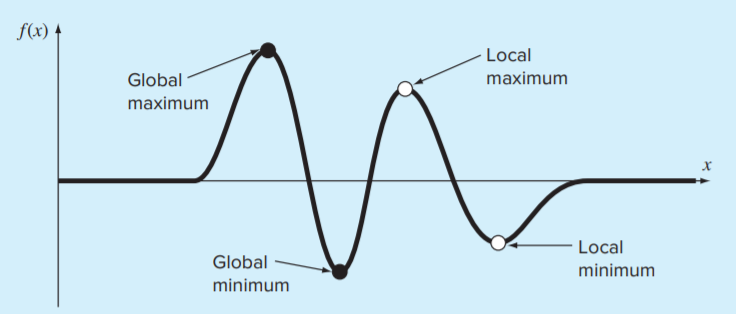
\includegraphics[width = 0.65\textwidth]{figures/localglobal}
		\end{figure}
		\begin{itemize}
			\item A \textit{global} optimum represents the very best solution. 
			\item A \textit{local} optimum, though not the very best, is better than its immediate neighbors. 
			\item Cases that include local optima are called \textit{multimodal}. 
			\item In such cases, we will almost always be interested in finding the global optimum.
			\item Therfore, we must be concerned about mistaking a local result for the global optimum. 
		\end{itemize}
		\item We will cover two methods for optimization - The \textit{golden section-search method} and the \textit{parabolic method}.
	\end{itemize}
\end{frame}

\begin{frame}[t]
\frametitle{1D Optimization}
\begin{itemize}
	\item In this unit we will cover techniques that find the minimum or maximum of a function of a single variable, i.e. $f(x)$.
	\item Just as finding the root location was complicated by the fact that several roots can occur for a single function, both local
	and global optima can occur in optimization.
	\begin{figure}
		\centering
		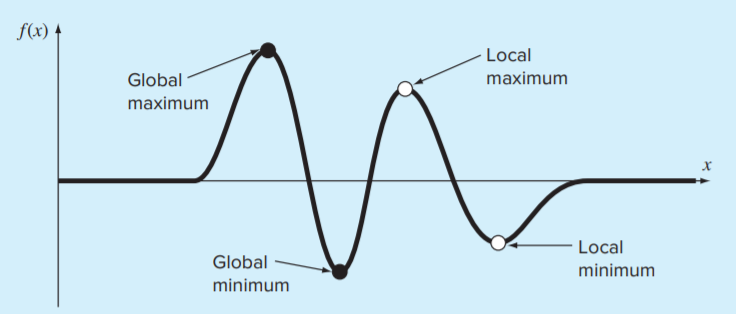
\includegraphics[width = 0.65\textwidth]{figures/localglobal}
	\end{figure}
	\begin{itemize}
		\item A \textit{global} optimum represents the very best solution. 
		\item A \textit{local} optimum, though not the very best, is better than its immediate neighbors. 
		\item Cases that include local optima are called \textit{multimodal}. 
		\item In such cases, we will almost always be interested in finding the global optimum.
		\item Therfore, we must be concerned about mistaking a local result for the global optimum. 
	\end{itemize}
    \item We will cover two methods for optimization - The \textit{golden section-search method} and the \textit{parabolic method}.
    \item Both of these methods can be considered \textit{Bracketing methods}.
\end{itemize}
\end{frame}

\section{The Golden-Section Search Method}

\begin{frame}[t]
	\frametitle{The golden-section search method}
	\begin{itemize}
		\item Like with Bisection, we need to define the interval that contains the optima.
	\end{itemize}
\end{frame}

\begin{frame}[t]
	\frametitle{The golden-section search method}
	\begin{itemize}
		\item Like with Bisection, we need to define the interval that contains the optima.
		\item We can us the same nomenclature we did with the Bisection method, letting $x_l$ be the lower bound and $x_u$ being the upper bound.
	\end{itemize}
\end{frame}

\begin{frame}[t]
	\frametitle{The golden-section search method}
	\begin{itemize}
		\item Like with Bisection, we need to define the interval that contains the optima.
		\item We can us the same nomenclature we did with the Bisection method, letting $x_l$ be the lower bound and $x_u$ being the upper bound.
		\item We cannot use a single intermediate value, $x_r$, like we did for Bisection, instead we need two intermediate values to detect whether a optima occurred.  \\\vspace{3pt}
	\end{itemize}
\end{frame}

\begin{frame}[t]
	\frametitle{The golden-section search method}
	\begin{itemize}
		\item Like with Bisection, we need to define the interval that contains the optima.
		\item We can us the same nomenclature we did with the Bisection method, letting $x_l$ be the lower bound and $x_u$ being the upper bound.
		\item We cannot use a single intermediate value, $x_r$, like we did for Bisection, instead we need two intermediate values to detect whether a optima occurred.  \\\vspace{3pt}
		\begin{minipage}{0.4\textwidth}
			\begin{itemize}
				\item The key to making this approach efficient is the wise choice of the intermediate points.
				\item For the golden-section search, the two intermediate points are chosen according to the golden ratio:
				$$x_1 = x_l + d $$
				$$x_2 = x_u - d $$
				Where
				$$d = (\Phi-1)(x_u-x_l)$$
				and the golden ratio $\Phi = 1.61803398874989 $.
			\end{itemize}
		\end{minipage}
		\begin{minipage}{0.5\textwidth}
			\begin{figure}
				\flushright
				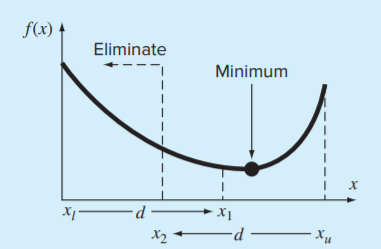
\includegraphics[width = .95\textwidth]{figures/methoda}
			\end{figure}
		\end{minipage}
	\end{itemize}
\end{frame}


\begin{frame}[t]
	\frametitle{The golden-section search method}
		\begin{minipage}{0.6\textwidth}
			\begin{itemize}
				\item For the golden-section search, the two intermediate points are chosen according to the golden ratio:
				$$x_1 = x_l + d $$
				$$x_2 = x_u - d $$
				Where $$d = (\Phi-1)(x_u-x_l)$$ and the golden ratio $\Phi = 1.61803398874989 $. \\\vspace{3pt}
				\item The function is evaluated at these two interior points. Two results can occur:
				\begin{itemize}
					\item If $f(x_1) < f (x_2)$, then $f (x_1)$ is the optima, and the domain of $x$ to the left of $x_2$, from $x_l$ to $x_2$, can be eliminated because it does not contain the optima. For this case, $x_2$ becomes the new $x_l$ for the next round.
					\item  If $f (x_2) < f (x_1)$, then $f (x_2)$ is the optima and the domain of $x$ to the right of $x_1$, from
					$x_1$ to $x_u$ would be eliminated. For this case, $x_1$ becomes the new $x_u$ for the next round.
				\end{itemize}
			\end{itemize}
		\end{minipage}
		\begin{minipage}{0.4\textwidth}
			\begin{figure}
				\centering
				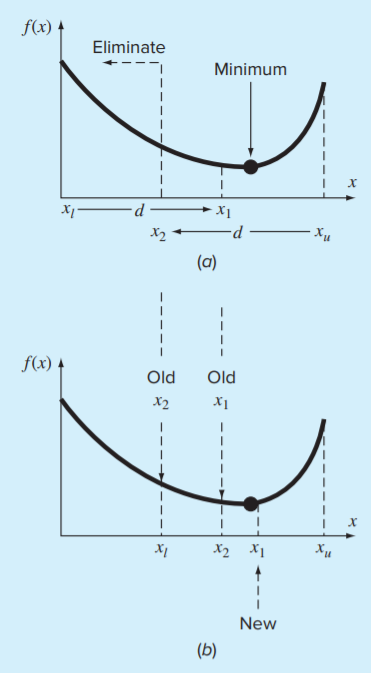
\includegraphics[width = 0.9\textwidth]{figures/method}
			\end{figure}
		\end{minipage}
\end{frame}

\begin{frame}
\frametitle{Example}
Let's find the minimum of 
$$f(x) = \frac{x^2}{10}-2\sin(x)$$
With and initial $x_l = 0$ and $x_u = 4$. \\\vspace{10pt}

\begin{minipage}{0.4\textwidth}
	The first thing we need to do is calculate the golden ratio that we use to create the two interior points:
	\begin{align*}
	d &= (1.61803-1)(4-0)\\
	 &=  2.4721
	\end{align*}
	Then our two interior points are 
	\begin{align*}
		x_1 &= x_l + d  = 0 + 2.4721 \\
		&= 2.4721 \\
		x_2 &= x_u - d \\  
		&= 4 - 2.4721 \\
		&= 1.5279\\
	\end{align*}
\end{minipage}
\begin{minipage}{0.6\textwidth}
	\begin{figure}
		\centering
		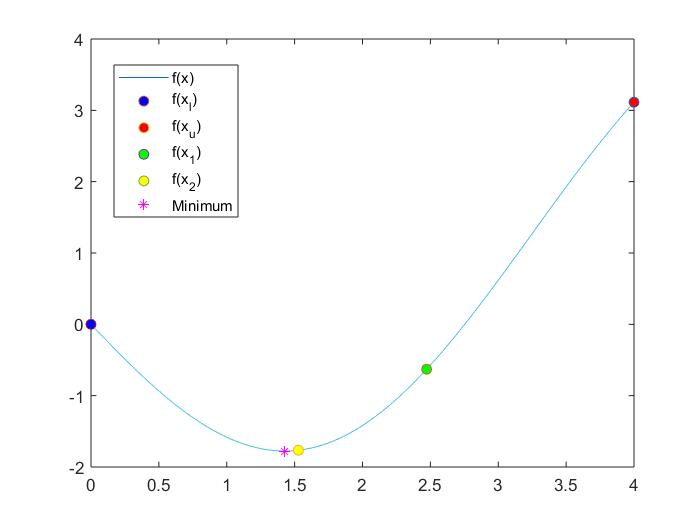
\includegraphics[width = 1.2\textwidth]{figures/iter1.jpg}
	\end{figure}
\end{minipage}
\end{frame}

\begin{frame}
	\frametitle{Example}
	\begin{minipage}{0.4\textwidth}
		Now we need to compute our function values and compare them to find our new domain
		\begin{align*}
			f(x_1) &= \frac{2.4721^2}{10}-2\sin(2.4721)\\
			&= -0.6300\\
			f(x_2) &= \frac{1.5279^2}{10}-2\sin(1.5279)\\
			& = -1.7647\\
		\end{align*}
		Now since $f(x_2)<f(x_1)$,
		$$ x_l = x_l $$
		$$ x_u \leftarrow x_1$$
		$$ x_1 \leftarrow x_2$$
		 
	\end{minipage}
	\begin{minipage}{0.6\textwidth}
		\centering
		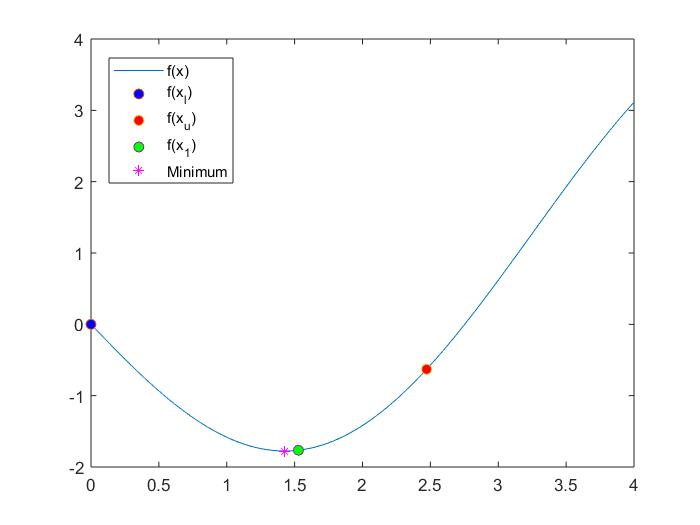
\includegraphics[width = 1.2\textwidth]{figures/iter1half.jpg}
	\end{minipage}	
\end{frame}

\begin{frame}
	\frametitle{Example}
	
	\begin{minipage}{0.4\textwidth}
		We now need to recalculate $d$
		\begin{align*}
			d &= 0.61803(x_u - x_l)\\
			 &=0.61803(2.4721 - 0)\\
			 &= 1.5279
		\end{align*}
		And define a new $x_2$
		\begin{align*}
			x_2 &= x_u - d\\
			&= 2.4721- 1.5279\\
			&= 0.9443
		\end{align*}

	\end{minipage}
	\begin{minipage}{0.6\textwidth}
		\centering
		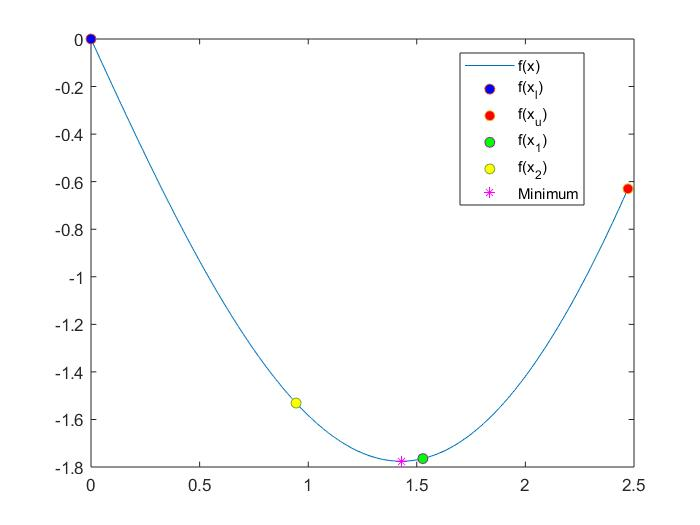
\includegraphics[width = 1.2\textwidth]{figures/iter2.jpg}
	\end{minipage}
\end{frame}

\begin{frame}
	\frametitle{Example}
	\begin{minipage}{0.4\textwidth}
		\textbf{Next iteration:} We need to compute our function values and compare them to find our new domain
		\begin{align*}
			f(x_1) &= \frac{1.5279^2}{10}-2\sin(1.5279)\\
			& = -1.7647\\
			f(x_2) &= \frac{0.9443^2}{10}-2\sin(0.9443)\\
			&= -1.5310\\
		\end{align*}
		Now since $f(x_1)<f(x_2)$,
		$$ x_u = x_u $$
		$$ x_l \leftarrow x_2$$ 
		$$ x_2 \leftarrow x_1$$
		
	\end{minipage}
	\begin{minipage}{0.6\textwidth}
		\centering
		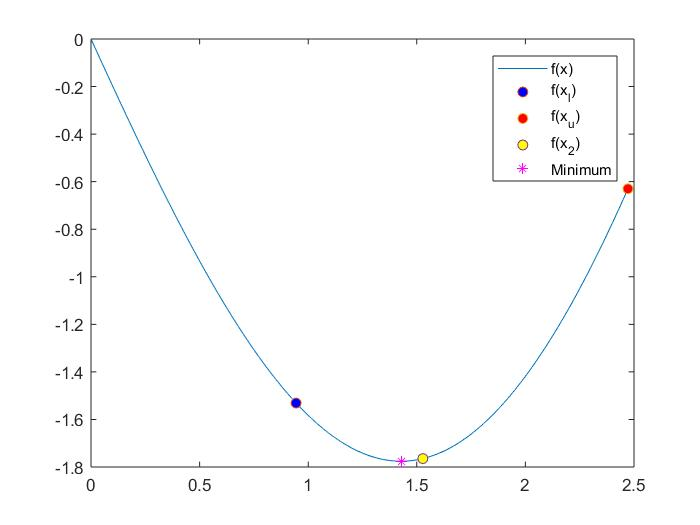
\includegraphics[width = 1.2\textwidth]{figures/iter2half.jpg}
	\end{minipage}	
\end{frame}

\begin{frame}
	\frametitle{Example}
	
	\begin{minipage}{0.4\textwidth}
		We now need to recalculate $d$
		\begin{align*}
			d &= 0.61803(x_u - x_l)\\
			&=0.61803(2.4721 - 0.9443)\\
			&= 0.9456
		\end{align*}
		And define a new $x_2$
		\begin{align*}
			x_1 &= x_l + d\\
			&= 0.9443 + 0.9456\\
			&= 1.8899
		\end{align*}
		
	\end{minipage}
	\begin{minipage}{0.6\textwidth}
		\centering
		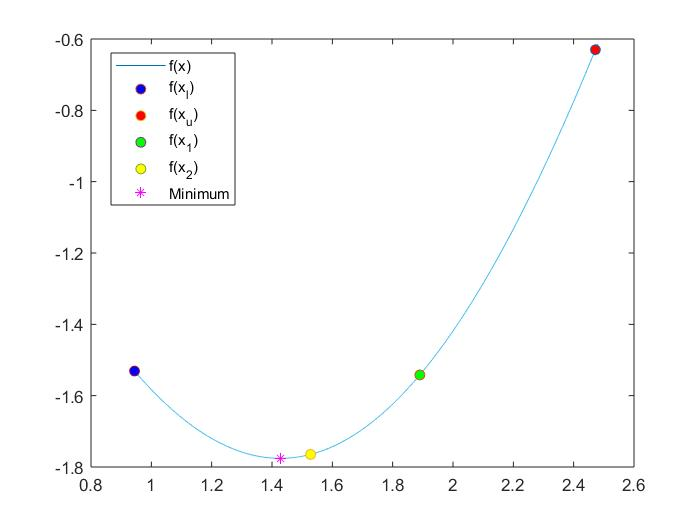
\includegraphics[width = 1.2\textwidth]{figures/iter3.jpg}
	\end{minipage}
Keep iterating until 
$$\epsilon_a = (2-\Phi)\left|\frac{x_u-x_l}{x_{opt}}\right| < tol$$
Where $x_{opt}$ is the new value of $x_1$ or $x_2$.
\end{frame}

\begin{frame}
	\frametitle{Sign-Off Activity}
	Now that you have an idea how this method works, write a pseudo code and post it to the \textbf{Golden-section search method} discussion board. You may sign-off once you've finished. 
\end{frame}

\end{document}
